\chapter{Trajectory Tracking} \label{Chapter1}
% Open problems
% introduce Pontryagin equations and talk about perturbation analysis

%%%%%%%%%%%%%%%%%
% PUT AS PLOT
% learning result on pendulum balance up

\section{Iterative Learning Control} \label{ILC}
% start with Arimoto 1984

Iterative Learning Control (ILC) was first introduced in \cite{Arimoto} as a reference tracking methodology that learns to track the trajectory through iterations of an identically repeated trial.
See \cite{Survey} for a detailed survey of the subject. Here we go briefly over a particular optimization-based ILC method that appeared recently in \cite{ILC_Angela}.

The method consists of two separate steps: \emph{disturbance estimation} and \emph{input update} steps. For disturbance estimation through iterations, a time-varying Kalman filter is designed. The estimated disturbance will then be fed in as input to the optimization step, where the control objective is formulated as a (constrained) convex optimization problem. 

\subsection{Lifted Domain Representation}\label{LiftedDomain}

It is assumed that a nominal model of the dynamical systems is available from the start. The nominal model dynamics

\begin{align}
\dot{\state}(t) &= f(\state(t), \sysInput(t), t) \\
\observations(t)       &= g(\state(t), t)
\end{align}

where $\state(t)$ is the state vector, and $\observations(t)$ the observation at time $t$, is first linearized around an a priori determined output trajectory $\observations^{*}(t)$:

\begin{align}
\dot{\tilde{\state}}(t) &= A(t)\tilde{\state}(t) + B(t)\tilde{\sysInput}(t) \label{linX} \\
\tilde{\observations}(t) &= C(t)\tilde{\state}(t) \label{linY}
\end{align}

where 

\begin{align}
A(t) &= \frac{\partial{f(\state(t), \sysInput(t), t)}}{\partial{\state}} \\
B(t) &= \frac{\partial{f(\state(t), \sysInput(t), t)}}{\partial{u}} \\
C(t) &= \frac{\partial{g(\state(t), t)}}{\partial{\state}}
\end{align}

are the Jacobians of $f$ and $g$ with respect to $\state$ and $\sysInput$. Here the tilde signs correspond to deviations from the reference trajectory and input:

\begin{align}
\tilde{\sysInput}(t) &= \sysInput(t) - \sysInput^{*}(t) \\
\tilde{\state}(t) &= \state(t) - \state^{*}(t) \\
\tilde{\observations}(t) &= \observations(t) - \observations^{*}(t)
\end{align}

See Appendix \ref{app:trjgen} for details on how to generate the reference input signal $\sysInput^{*}(t)$ given output signal $\observations^{*}(t)$.

For a fixed discretization $h$, assuming a constant input signal between times $t$, and $t+h$ (also known as \emph{zero-order hold} in the control community), we can discretize the equations (\ref{linX}) and (\ref{linY}) as follows:

\begin{align}
\tilde{\state}(k+1) &= A_{D}(k)\tilde{\state}(k) + B_{D}(k)\tilde{\sysInput}(k) \label{discX} \\
\tilde{\observations}(k+1) &= C_{D}(k+1)\tilde{\state}(k+1) \label{discY}
\end{align}

These discretized matrices are 

\begin{align}
A_{D}(k) &= e^{A(k)h} \label{discrA} \\
B_{D}(k) &= A^{-1}(k)(A_{D}(k) - I)B(k) \label{discrB} \\
C_{D}(k) &= C(k)
\end{align}

(\ref{discrA}) and (\ref{discrB}) can be efficiently implemented by noting:

\begin{equation*}
\exp^{h \left(
\begin{BMAT}(rc){c:c}{c:c}
A(k) & B(k) \\
0 & 0
\end{BMAT} 
\right)}
= 
\left(
\begin{BMAT}(rc){c:c}{c:c}
A_{D}(k) & B_{D}(k) \\
0 & I
\end{BMAT} 
\right)
\end{equation*}

After discretization, the vectors $\tilde{\sysInput}$, $\tilde{\state}$, and $\tilde{\observations}$ can be stacked together to form the lifted vector representation of the dynamics:

\begin{align}
\state &= F\sysInput + d^{0} \label{liftedX} \\
\observations &= G\state \label{liftedY}
\end{align}

Here the lifted matrix is a block matrix of the following form:

\begin{equation}
F = 
\left(
\begin{array}{ccc}
F_{(1,1)} & \ldots & F_{(1,N)} \\
\vdots & \ddots & \vdots \\
F_{(N,1)} & \ldots & F_{(N,N)} 
\end{array} \right)
\end{equation}

where each entry is as follows:

\begin{equation}
F_{(i,j)} = 
\left\{
\begin{array}{cccc}
A_{D}(i-1) & \dotsi & A_{D}(j)B_{D}(j-1) & \text{if } j < i,\\
B_{D}(j-1) & & & \text{if } j = i,\\
0 & & & \text{if } j > i.
\end{array} 
\right\}.
\end{equation}

The matrix $G$ is only block diagonal, with entries consisting of $C_{D}$ matrix stacked diagonally.
The vector $d^{0}$ is the \emph{free response} of the system to the initial deviation $\tilde{\state}(0)$. The initial deviation from the reference trajectory $\state^{*}(t)$ is the only disturbance in this model. The static linear mapping (\ref{liftedX}) - (\ref{liftedY}) is a useful formulation for ILC, since each iteration can be described succinctly in this way. Extending it to many iterations, indexed by $l$, and more general disturbances (due to unmodeled dynamics, parameter mismatch, etc.) we get:

\begin{align}
\state_{l} &= F\sysInput_{l} + d_{l} + N_{\xi}\xi_{l} \label{liftedXiter} \\
\observations_{l} &= G\state_{l} + N_{\nu}\nu_{l} \label{liftedYiter} \\
d_{l} &= d_{l-1}	+ \omega_{l-1} \label{dEvolution}	
\end{align}

\subsection{Disturbance estimation}
\label{ILC_Kalman}

The process noise signal $\xi$ in (\ref{liftedXiter}) and the measurement noise signal $\nu$ in (\ref{liftedYiter}) are both zero-mean Gaussian white noise with unit variance, $\xi, \nu \sim \mathcal{N}(0,1)$.
(\ref{dEvolution}) is a model describing the evolution of the disturbance. This model is necessary in order to approach the problem from the standard Kalman filter perspective. The dynamics of the disturbance is then as follows:

\begin{equation}
\begin{aligned}
d_{l} &= d_{l-1}	+ \omega_{l-1} \\
\observations_{l} &= Gd_{l} + GF\sysInput_{l} + \mu_{l} \label{DisturbanceDynamics}
\end{aligned}
\end{equation}

Here $\omega_{l} \sim \mathcal{N}(0, M_{l})$ is just another zero-mean Gaussian white noise signal, modelling a slight variation in $d$. For a critique of this approach, see section \ref{critique}. The output noise in (\ref{DisturbanceDynamics}) is the stacking of process and noise signals, i.e. $\mu = G N_{\xi}\xi_{l} + N_{\nu}\nu_{l}$, $\mu_{l} \sim \mathcal{N}(0, \Omega_{l})$. 

% Kalman filter update equations
% refer to article for tuning covariance matrices for faster/better range of convergence.
Kalman filter update equations for the dynamics given in (\ref{DisturbanceDynamics}) are as follows:

\begin{align}
S_{l} &= P_{l-1} + \Omega_{l-1} \\
K_{l} &= S_{l}G^{\mathrm{T}}(GS_{l}G^{\mathrm{T}} + M_{l})^{-1} \\
P_{l} &= (I - K_{l}G)S_{l}
\label{Kalman}
\end{align}

Here $P_{l} = E[(d_{l} - \hat{d}_{l})(d_{l} - \hat{d}_{l})^{\mathrm{T}}]$ is the covariance of the disturbance $d_{l}$. If $P_{0}$ and $\hat{d}_{0}$ are provided as initial values, the Kalman filter will update the Kalman gain $K_{l}$ at each iteration and estimate $d_{l}$ as:

\begin{equation}
\hat{d}_{l} = \hat{d}_{l-1} + K_{l}(\observations_{l} - G\hat{d}_{l-1} - GF\sysInput_{l})
\end{equation}

The performance of the estimation is dependent on the design parameters, the covariance matrices $\Omega_{l}, M_{l}$ and initial values $P_{0}$ and $\hat{d}_{0}$. More information on the tuning of such parameters can be found in \cite{ILC_Angela}. 

\subsection{Input Update}

In the input update step, the objective is to find the next control input difference $\sysInput_{l+1}$ which will compensate for the estimated disturbance in some optimal sense. Then the total applied input in the next iteration will be $\sysInput(t) = \sysInput^{*}(t) + \sysInput_{l+1}(t)$. Here, the expected value of the deviation from the reference trajectory 

\begin{equation}
E[\state_{l+1}|\observations_{1}, \ldots, \observations_{l}] = F\sysInput_{l+1} + \hat{d}_{l}
\end{equation}

is to be minimized, i.e. the following optimization problem is solved at each step:

\begin{equation}
\begin{aligned}
\sysInput_{l+1} &= \argmin_{\sysInput} ||F\sysInput + \hat{d}_{l}||_{2} \\ 
& \text{subject to } L\sysInput \leq q
\end{aligned}
\end{equation}

Refer to the article \cite{ILC_Angela} for additional tuning such as derivative norm penalties, optimization under different norms, and scaling for better and smoother performance. Constraint $L, q$ formulation is not given here but constraints can be transformed around the reference trajectory, discretized and formed into the \emph{lifted vector representation} along with the process detailed in \ref{LiftedDomain}.

\subsection{Analysis of the method}\label{critique}

% % % % % % % % % % % % % % % % %
% critique: the Kalman filter approach is wrong
The method works very well in cases where the nominal model of the dynamical system under consideration is not far off from the real dynamics of the system. In this case the method will converge in very few iterations. The performance of the method is presented in the results section \ref{Results1} in two example problems. However the proposed standard Kalman filter approach is an \emph{ad hoc} solution to the estimation problem and will not be effective in estimating large disturbances. To see this, let us consider a more complete description of the system, denoted as \emph{real}:

\begin{align}
\dot{\state}(t) &= f_{real}(\state(t), \sysInput(t), t) \\
\end{align}

This system can also be linearized around a reference trajectory $\state^{*}(t)$, discretized, and then \emph{lifted} to form the lifted-vector representation. Assuming, for simplification, that the states themselves are fully observed, i.e. $\observations(t) = \state(t)$, and stacking process and measurement noises in $\mu$ we obtain:

\begin{align}
\state_{l} &= F_{nom}\sysInput_{l} + d_{l} + \mu_{l} \label{liftedXiterNom} \\
d_{l} &:= \Delta F \sysInput_{l} = (F_{real}-F_{nom})\sysInput_{l} \label{dEvolutionReal}	
\end{align}

Here $d_{l}$ in (\ref{dEvolutionReal}) cannot be estimated by a Kalman filter because the matrix $\Delta F$ is not known. Instead the matrix $\Delta F$ should be estimated from the previous iteration results:

\begin{align}
\mathbf{v}_{l} &:= \state_{l} - F_{nom}\sysInput_{l} \\
\mathbf{v}_{l} &= \Delta F \sysInput_{l} + \mu_{l}
\end{align}

The matrix should hence be estimated from noisy outputs $\mathbf{v}_{l}$ and inputs, where $\sysInput_{l}$, $l = 1, \ldots, N$, and $N$ the total number of iterations up to the estimation. The problem falls under the category of \emph{exploration-exploitation} because simultaneously while estimation of the matrix difference $\Delta F$ is critical, the real objective is to the drive the deviation signal $\state_{l}$ to zero.

% mention perhaps the special sparse structure of deltaF

Another important problem with the method is the linearization around a reference trajectory. This linearization is only accurate for small disturbances around the trajectory, and will prevent the method from converging under wider model mismatches. An important research topic would be to characterize under which conditions the method converges and consider whether it is possible to still achieve learning feed-forward control signals \emph{without} linearizing around a trajectory.

% on stability and safety
% limitations
As a final point, note that stability is also not guaranteed with this method. In fact, it is assumed that the motion of the system stays close to the reference trajectory during the learning process and has to be enforced otherwise by stopping and restarting the whole iteration.

% % % % % % % % % % % % % % % % % 
These considerations all lead us away from ILC and into machine learning methodologies adapted to control, one of which is the learning algorithm CGP-UCB introduced in \ref{ContextBandit}.

%\section{Model Predictive Control}
% present the main idea behind MPC.
% approximating the value function
% learning result on 2-d robot kinematics with ILC as comparison

\section{Problem Setting and Methodology} 
\label{methodology}
%%%%%%%%%%%%%%%%%
% Include the derivation of example delta J

\subsection{Optimal Control}
% references needed!!!
Consider the following system dynamics: 

\begin{equation}
\dot{\state}_t = f(\state_t,\sysInput_t), \quad  t \geq 0,
\label{eq:readDynamics}
\end{equation}

where $\state_t \in \mathbb{R}^n$ denotes the state of the system at time $t$ and $\sysInput_t \in \mathbb{R}^m$ denotes the control input.  

In continuous time optimal control, the control objective at time $\tau, \, 0 \leq \tau \leq T$ can be given as follows:

% % % % Add the terminal cost
\begin{equation}
\begin{aligned}
\sysInput^{*}(t) &= \argmin_{\sysInput \in D} J(\sysInput) \quad \text{subject to} \\
\dot{\state}_t &= f(\state_t,\sysInput_t), \quad  t \geq \tau
\end{aligned}
\label{optimalControl}
\end{equation}

where $J(\sysInput)$ is the cost functional defined by:

\begin{equation}
J(\sysInput) = \int\limits_{t = \tau}^{T} (\state(t) - \state^{*}(t))^{\mathrm{T}}Q(t)(\state(t) - \state^{*}(t)) + \sysInput(t)^{\mathrm{T}}R(t)\sysInput(t) \label{costFunctional}
\end{equation}

$D$ denotes the constraints imposed on the dynamics. $Q$ and $R$ are matrices penalizing the deviations from the defined trajectory and the control input, respectively. They are generally taken to be diagonal with constant nonnegative entries. Zero diagonal entries correspond to states that are not actively tracked. In the limit as $T$ goes to infinity, the optimization in (\ref{costFunctional}) becomes the infinite-horizon optimal control problem. In this case $Q(t)$ and $R(t)$ must be decaying sufficiently fast to make $J(\sysInput)$ finite. 

% reference needed
A necessary condition for a control signal $\sysInput(t)$ to be an optimal solution of (\ref{optimalControl}) is that it should satisfy \emph{Pontryagin's minimum principle}. A necessary and sufficient condition is that $\sysInput(t)$ should be a solution of the \emph{Hamilton-Jacobi-Bellman} (HJB) partial differential equation \cite{Bertsekas:DP01}.

Assuming zero-order hold and an Euler discretization of (\ref{costFunctional}), we get the following:

\begin{equation}
J(\sysInput) = \sum\limits_{i = \tau_{h}}^{N} (\state_{i} - \state_{i}^{*})^{\mathrm{T}}Q(\state_{i} - \state_{i}^{*}) + \sysInput_{i}^{\mathrm{T}}R\sysInput_{i} \label{costDiscrete}
\end{equation}

where $\tau_{h} \geq \tau/h$ is the next time stage under the discretization $h = T/N$. From now on we will consider $R$ to be zero and only concentrate on the costs caused by the trajectory deviations. Rewriting (\ref{costDiscrete}) in a more convenient form:

\begin{equation}
J(\sysInput) = \sum\limits_{i = \tau_{h}}^{N} ||\state_{i} - \state_{i}^{*}||_{Q}^{2} \label{costNormed}
\end{equation}

A solution $\sysInput(t)$ of this discrete formulation should satisfy Bellman's equations, the discrete form of the HJB equations. In the finite horizon case, this solution can be calculated recursively using Dynamic Programming, and in the infinite-horizon case, using Policy Iteration or Value Iteration algorithms. See \cite{Bertsekas:DP01} for details. These algorithms all suffer from the \emph{curse of dimensionality} and they are computationally very inefficient in high-dimensional state spaces. This is because they have to consider \emph{non-greedy} policies to calculate an optimal solution. Non-greedy policies can be avoided in cases where the desired trajectory $\state^{*}(t)$ is always \emph{feasible}. More precisely, we have the following: \\

% which assumptions can we remove/relax ?
\begin{proposition}[Dissociation of stage costs]
The finite horizon optimal control problem with the cost given in (\ref{costNormed}) under zero-noise assumption\footnote{Here we include any unknown dynamics as a disturbance that contributes to the noise signal.} reduces to sequential greedy stage-cost minimization given that the trajectory $\state^{*}(t)$ is \emph{feasible} throughout, i.e. $\forall t \ \ \exists \sysInput \ \ s.t. \ \ \state^{*}(t+h) = f_{h}(\state(t), \sysInput(t), t)$.
\label{Prop:1}
\end{proposition}

\begin{proof}
The proof is trivial. First we note that the finite horizon optimal control problem under the zero-noise assumption can be posed as a non-stochastic \emph{shortest path problem} which can be solved iteratively instead of recursively. At time stage $t \ $:

\begin{equation*}
J^{*}_{t}(\sysInput_{t:N}) = \min_{u_{t}}(J_{t}(u_{t}) + J^{*}_{t+1}(\mathbf{U}_{t+1:N}))
\end{equation*}

where $\sysInput_{t:N} = (u_{t}, \ldots, u_{N})$, future inputs stacked together. Since each $J_{t}(u_{t}) = 0$ due to the feasibility assumption for all $t$, the optimal cost to go $J^{*}_{t}(\sysInput_{1:N}) = 0$. But we can always achieve this cost by minimizing the stage cost $J_{t}(\sysInput_{t}) = 0$ greedily.

\end{proof}

Here $f_{h}$ is the discretized version of (\ref{eq:readDynamics}):

\begin{equation}
\state_{t+h} = f_{h}(\state(t), \sysInput(t), t) = \state_{t} + \int_{t}^{t+h}f(\state_{t'},\sysInput_t)dt' \label{eq:realDynamics_discrete}
\end{equation}

Zero-noise including the perfectly known model assumption in Proposition \ref{Prop:1} is obviously too stringent. Here we conjecture that this assumption can be somewhat relaxed and the proposition will still hold, at least in a probabilistic sense. If it is possible to put a probabilistic bound on the noise and the deviation due to model mismatch, then we can plan feasible (with high probability) trajectories on the state space with these bounds in mind, and still expect to achieve good performance with a greedy optimization. More precisely, in terms of \emph{stability} theory, we would like to stabilize the system dynamics around the trajectory.

% % % % update on this
\subsection{Stability}
\label{stability}
If the tracked states deviate by a large margin from the desired trajectory during an initial run, the next state to go to, $\state^{*}_{t+h}$ will have to be recalculated instead to avoid violating input constraints. Given a trajectory of horizon of size $T$ and a method $H(\state(t), \state^{*}(t+h), \ldots, \state^{*}(t+Th))$ for calculating a converging trajectory over the horizon:
\begin{equation}
\state^{*}_{new}(t+h) = H(\state(t), \state^{*}(t+h), \ldots, \state^{*}(t+Th)) \label{converging_trj} \\
\end{equation}
This method $H$ can be used to speed up the convergence of the proposed method over time. 
Of course since the disturbance dynamics is not known exactly, such a method can only generate \emph{feasible} converging trajectories probabilistically. Over time however, the disturbance dynamics will be more or less known around the traversed state-space points, and converging trajectories will be asymptotically stable with high probability (w.h.p.). We have the following:

% first attempt at proposition
% add CGP-UCB assumptions: that the cost function is a GP with known parameters, or known RKHS bound
\begin{proposition}[Stability]
Assume that we have a method $H$ that can compute converging trajectories w.h.p. $p \leq 1 - \delta_{1}$. If this method incurs over time $T$ cumulative regret on the order $\mathcal{O}(T^{\alpha})$, $\alpha < 1$ w.h.p. $p \leq 1 - \delta_{2}$, then for the inputs calculated using CGP-UCB, the dynamics is asymptotically stable w.h.p. $p = 1 - \delta, \, \delta \geq \delta_{1} + \delta_{2}$.
\label{Prop:1}
\end{proposition}

\begin{proof}
Since regret at time stage $t$ is $r_{t} = J(\sysInput_{t}) - J(\sysInput^{*})$, where $\sysInput^{*} = \operatorname*{arg\,min}_{u \in U(t)} \|\state_{t+h} - \state^{*}_{t+h}\|_{Q}^{2}$, the cumulative regret at time stage $T$:

\begin{equation}
R_{T} = \sum_{t=1}^{T}r_{t} = \sum_{t=1}^{T}J(\sysInput_{t}) - J(\sysInput^{*}) \label{cumRegret}
\end{equation}

$R_{T}$ is of order $\mathcal{O}(T^{1/2})$ w.h.p $1-\delta_{1}$, hence assuming that the method $H$ incurs regret of order $\mathcal{O}(T^{\alpha})$, $\alpha < 1$ w.h.p $1-\delta_{2}$, the regret for $H$ being defined by:

\begin{equation}
r_{t}^{\mathrm{H}} = J(\sysInput^{*}|\state^{*}_{t+h}) - J(\sysInput^{*}|\state^{\mathrm{H}}_{t+h})
\end{equation}

where $\state_{t+h}^{\mathrm{H}}$ is any feasible next state such that $J(\sysInput^{*}|\state_{t+h}^{\mathrm{H}}) = 0$, then the total cost to go

\begin{align}
\sum_{t=1}^{T}J(\sysInput_{t}) &= \sum_{t=1}^{T}\Delta\state^{\mathrm{T}}Q\Delta\state = \mathcal{O}(T^{\beta}), \\ & \text{w.h.p. } 1 - \delta, \quad \delta \geq \delta_{1} + \delta_{2} \\
\beta &= \max(1/2, \alpha) < 1
\end{align}

This implies that $\lim_{T \to \infty} \Delta\state^{\mathrm{T}}Q\Delta\state = 0$ w.h.p. For positive definite $Q \ $, $\lim_{T \to \infty} \Delta\state = 0$ w.h.p.

\end{proof}

Here method $H$ acts as a magnet around the trajectory, making sure that the trajectories do not deviate over time $T$ by more than $\mathcal{O}(T^{\alpha})$. $H$ can be constructed by noting \eqref{function bound}: converging trajectories should be chosen such that the uncertainty is smallest. This task gets easier as the variance $\sigma^{2}$ decreases over time.

%converging trajectories
\subsection{Stage Cost Minimization}
\label{StageCostMin}

The control objective at time $t$ is to track the desired state at the next time step $\state^{*}_{t+h}$, that is minimizing the following stage cost:

\begin{equation}
J_{t} := \|\state_{t+h} - \state^{*}_{t+h}\|_{Q}^{2}. \label{eq:stagecost}
\end{equation}

Furthermore, assume a nominal model of the system given in (\ref{eq:readDynamics}) is known and given by

\begin{equation}
\dot{\state}_t = f_{\mathrm{nom}}(\state_t,\sysInput_t) \label{nominal_model} \\.
\end{equation}

Note that the above nominal model is typically derived from first principles. This nominal model is only an approximation of (\ref{eq:readDynamics}) and the unmodelled dynamics can be seen as repeating disturbances that can be learned using the CGP-UCB framework introduced in \ref{ContextBandit}.

Tracking the global minimum of the stage cost (\ref{eq:stagecost}) results in solving the following optimization problem at each time step:

\begin{equation}
\begin{aligned}
\sysInput_{t} &= \operatorname*{arg\,min}_{u \in U(t)}\|\state_{t+h} - \state^{*}_{t+h}\|_{Q}^{2} \\
\state_{t+h} &= \state_{t} + \int_{t}^{t+h}f(\state_{t'},\sysInput_t)dt'
\end{aligned}
\label{stageCostOptim}
\end{equation}

where $U(t) \subset \mathbb{R}^m$ is the feasible input space at time step $t$, assuming zero-order hold. But system dynamics $f$ in (\ref{stageCostOptim}) is not known. However, since we have a nominal model, we can learn $f$ indirectly by just learning the difference in cost predicted by the nominal model and the actual cost:

\begin{equation}
\|\state_{t+h} - \state^{*}_{t+h}\|_{Q}^{2} - \|\hat{\state}_{t+h} - \state^{*}_{t+h}\|_{Q}^{2} \label{eq:deltaJ}
\end{equation}

where 
\begin{equation}
\hat{\state}_{t+h} = \state_{t} + \int_{t}^{t+h}f_{\mathrm{nom}}(\state_{t'},\sysInput_t)dt' \label{eq:nominal_discrete}
\end{equation}

is the predicted state using the nominal model.

The above cost given in (\ref{eq:deltaJ}) can also be rewritten to show explicit dependence on context and repeating disturbances:

\begin{align}
\Delta J_{t} &: (\state_t, \state^{*}_{t+h}; \sysInput_t) \mapsto \Delta F^{\mathrm{T}} Q \Delta F + 2(\hat{\state}_{t+h} - \state^{*}_{t+h})^{\mathrm{T}} Q \Delta F \label{delta_cost} \\
\Delta F &:= \int_{t}^{t+h}f(\state_{t'},\sysInput_t)dt' - f_{\mathrm{nom}}(\state_{t'},\sysInput_t)dt' \label{delta_f} 
\end{align}

where $\state_t \times \state^{*}_{t+h} \in C$, the context space, and $\sysInput_t \in U(t)$. This whole process, in terms of the CGP-UCB optimization, translates into adding the nominal model predicted cost $\|\hat{\state}_{t+h} - \state^{\mathrm{*}}_{t+h}\|_{Q}^{2}$, a known function of $\sysInput$, as a prior mean in (\ref{ucb}):

\begin{equation}
\sysInput_{t} = \operatorname*{arg\,min}_{u \in U(t)} \left\lbrace  \|\hat{\state}_{t+h} - \state^{*}_{t+h}\|_{Q}^{2} \right. 		+ \mu(\sysInput;\context) - \beta_t^{1/2}\sigma(\sysInput;\context) \rbrace \label{boostedUCB}
\end{equation}

This known component of the mean function thus does not have to be estimated during hyperparameter estimation. We believe the performance of the proposed method is very sensitive to changes in the mean function parameters, and hence by adding the nominal cost, we are ensuring more robustness with respect to hyperparameter estimation. 

\subsection{Examples}
\label{examples}
% here examples from the quadrocopter
As an example consider the quadrocopter model. A two-dimensional model of the quadrocopter dynamics derived from first principles can be given as follows \cite{ILC_Angela}:

\begin{equation}
\begin{aligned}
\ddot{y} &= -f_{\mathrm{coll}} \sin\phi \\
\ddot{z} &=  f_{\mathrm{coll}}\cos\phi - g \\
\dot{\phi} &= \omega_{x}
\end{aligned}
\label{quadrocopterDynamics}
\end{equation}

where state $\state = (y,\dot{y},z,\dot{z},\phi)$. The states $y, z$ are trajectories to be tracked, corresponding to the horizontal and vertical axes and the control input $\sysInput = (f_{\mathrm{coll}}, \omega_x)$, where $f_{\mathrm{coll}}$ is the collective thrust and $\omega_x$ is rate of change of the angle of attack with respect to the x-axis. Constraints are given in Appendix \ref{app:trjgen}, see Table \ref{table_parameters} and (\ref{thrust_constraints}) -- (\ref{angular_vel_constraints}). 

Unmodeled dynamics in quadrocopters could be due to parameter mismatch (e.g. gravity difference) or a more general repeating disturbance (e.g. a fan).

\textit{Example 1}. As an analytical example consider a quadrocopter operating in another planet, whose nominal model represents the quadrocopter flying in Earth. Gravity difference $\Delta g$ using Euler discretization (with time discretization $h$) and $Q$ as the identity matrix, causes the following cost difference at each time stage:

\begin{equation}
\Delta J(\state,\state^{*};\sysInput) = h^{2}(\Delta g)^{2} - 2h^{2}g\Delta g + 2h\Delta g(s_{4}-s^{*}_{4}) + 2h^{2}\Delta g u_{1} \cos s_{5} \label{example1General} 
\end{equation}

In Mars, the huge gravity difference ($g_{mars} = 3.75, g_{earth} = 9.81$), and $h = 0.02$ causes the following cost difference:

\begin{equation*}
-0.0329 + 0.2424(s_{4} - s^{*}_{4}) + 0.0048u_{1}\cos s_{5} \label{exampleMars} 
\end{equation*}

where $s_{4}$ is the $\dot{z}(t)$, $s_{5}$ is $\dot{\phi}(t)$, $s^{*}_{4}$ is the $\dot{z}(t+h)$ along the trajectory and $u_{1}$ is the collective thrust $f_{\mathrm{coll}}$. We effectively learn this function $\Delta J(\state, \state^{*}; \sysInput): \mathbb{R}^{3} \times \mathbb{R} \mapsto \mathbb{R}$, as we do online CGP-UCB optimization along the trajectory.

\textit{Example 2}. As another example consider the effect of constant wind on the quadrocopter operation. Assuming the wind, coming at an angle of $\theta$ from the horizontal axis, exerts a pressure $P_{wind}$ on the quadrocopter with area $A$, the dynamics (\ref{quadrocopterDynamics}) is modified as follows: 

\begin{align}
\ddot{y} &= -f_{\mathrm{coll}} \sin\phi \label{yddot} + P_{wind} A sin(\theta + \phi) cos \theta \\
\ddot{z} &=  f_{\mathrm{coll}} \cos\phi - g \label{zddot} + P_{wind} A sin(\theta + \phi) sin \theta \\
\dot{\phi} &= \omega_{x} \label{phidot}
\end{align}

The cost difference (again using Euler discretization and identity matrix for $Q$) is shown below:

\begin{equation}
\begin{aligned}
& \Delta J(\state,\state^{*};\sysInput) = h^{2}P_{wind}^{2}A^{2} \sin^{2}(s_{5} + \theta)  \\
& \hspace*{2em} + 2hP_{wind}A\sin(s_{5} + \theta)((s_{2} - s^{*}_{2})\cos\theta + (s_{4} - s^{*}_{4})\sin\theta)  \\
& \hspace*{2em} - 2h^{2}P_{wind}Au_{1}\sin(s_{5} - \theta)\sin(s_{5} + \theta) \\
& \hspace*{2em} - 2h^{2}P_{wind}Ag\sin\theta\sin(s_{5} + \theta) 
\end{aligned}
\label{example2General}
\end{equation}

Assuming a perfectly horizontal wind, i.e. $\theta = 0$, cost difference is simplified:

\begin{align}
\Delta J(\state,\state^{\mathrm{*}};\sysInput) = (h^{2}P_{wind}^{2}A^{2} - 2h^{2}P_{wind}A\ u_{1}) \sin^{2} s_{5} + 2hP_{wind}A(s_{2} - s^{*}_{2})\sin s_{5} \label{QuadTheta0}
\end{align}
%

\subsubsection*{Derivation}
%%% Here put the derivation of the 2nd example and tie in with the 1st
(\ref{example2General}) can be derived using the stage cost difference equation (\ref{delta_cost}):

\begin{equation}
\begin{aligned}
\Delta J &= h^{2}\begin{pmatrix} 0 \\ P_{wind} A \sin(\theta + \phi) \cos \theta \\ 0 \\ P_{wind} A \sin(\theta + \phi) \sin \theta \\ 0
\end{pmatrix}^{\mathrm{T}}\begin{pmatrix} 0 \\ P_{wind} A \sin(\theta + \phi) \cos \theta \\ 0 \\ P_{wind} A \sin(\theta + \phi) \sin \theta \\ 0
\end{pmatrix} + \\
& \quad 2h(\hat{\state}_{t+h} - \state^{*}_{t+h})^{\mathrm{T}}\begin{pmatrix} 0 \\ P_{wind} A \sin(\theta + \phi) \cos \theta \\ 0 \\ P_{wind} A \sin(\theta + \phi) \sin \theta \\ 0
\end{pmatrix} \\
&= h^{2}P_{wind}^{2}A^{2}\sin^{2}(\theta + \phi) + 2h \begin{pmatrix} 0 \\ \Delta \dot{y} - hf_{\mathrm{coll}} \sin(\phi) \\ 0 \\ \Delta \dot{z} + hf_{\mathrm{coll}} \cos(\phi) - hg \\ 0 \end{pmatrix}^{\mathrm{T}}  \begin{pmatrix} 0 \\ P_{wind} A \sin(\theta + \phi) \cos \theta \\ 0 \\ P_{wind} A \sin(\theta + \phi) \sin \theta \\ 0 \end{pmatrix} \\
&= h^{2}P_{wind}^{2}A^{2}\sin^{2}(\theta + \phi) + 2hP_{wind}A \sin(\theta + \phi)(\Delta \dot{y} \cos\theta + \Delta \dot{z} \sin\theta) - \\ 
& \quad 2h^{2}P_{wind}Af_{\mathrm{coll}}\sin(\phi - \theta)\sin(\phi + \theta) - 2h^{2}P_{wind}Ag \sin(\theta + \phi) \sin\theta 
\end{aligned}
\label{derivationQuad}
\end{equation}

If $\theta = 0$ then all terms with $\sin \theta$ disappear, and we're left with (\ref{QuadTheta0}). If $\theta = \pi/2$ then (\ref{derivationQuad}) reduces to:

\begin{equation}
\Delta J = h^{2}P_{wind}^{2}A^{2}\cos^{2}\phi + 2hP_{wind}A\cos\phi(\Delta \dot{z} - hg) + 2h^{2}P_{wind}Af_{\mathrm{coll}}\cos^{2}\phi
\end{equation}

The acceleration is due to the wind force $P_{wind}A\cos\phi$. Replacing it with $\Delta g$,  we get 
(\ref{example1General}).

\section{Implementation}
\label{Implementation}
The process is summarized in Figure \ref{alg} in algorithmic form.

\begin{figure}[!hbp]
\begin{algorithmic}[1]
\REQUIRE $n$ example trajectories
\FOR{$i=1$ to $n$}
	\STATE $\Delta J(t) \leftarrow \|\state_{t+h} - \state^{\mathrm{*}}_{t+h}\|_{2}^{2} - \|\hat{\state}_{t+h} - \state^{\mathrm{*}}_{t+h}\|_{2}^{2} $
\ENDFOR
\STATE Search through models and fit hyperparameters
\LOOP[for a new trajectory]
	\FOR{$t=1$ to $T$}
		\STATE $\beta_{t} \leftarrow \beta(t,\delta, d, a, b, r)$
		\STATE $\context := (\state_t, \state^{*}_{t+h})$
		\STATE $\sysInput_{t} = \operatorname*{arg\,min}_{\sysInput \in U(t)} \left\lbrace  \|\hat{\state}_{t+h} - \state^{*}_{t+h}\|_{Q}^{2} \right. 		+ \mu(\sysInput;\context) - \beta_t^{1/2}\sigma(\sysInput;\context) \rbrace $
		\STATE $\state_{t+h} \leftarrow \state_{t} + \int_{t}^{t+h}f(\state,\sysInput_{t})dt'$
		\STATE $\Delta J(\sysInput_{t}) \leftarrow \|\state_{t+h} - \state^{*}_{t+h}\|_{Q}^{2} - \|\hat{\state}_{t+h} - \state^{*}_{t+h}\|_{Q}^{2} $
		\STATE Update GP (\ref{gpUpdate_mu}), (\ref{gpUpdate_sigma}) with $(\sysInput_{t}, \Delta J(\sysInput_{t}))$
	\ENDFOR
\ENDLOOP
\end{algorithmic}
\caption{CGP-UCB for trajectory tracking}
\label{alg}
\end{figure}

Before starting GP-optimization, we need to train the GP by estimating hyperparameters from gathered data. Hence the process starts in lines 1-3 with gathering the necessary evaluations for hyperparameter estimation from trial trajectory runs, i.e. contexts, actions, and cost differences. 

As mentioned in \ref{StageCostMin}, the current state and the desired next state constitute the contexts, $\ \state_t \times \state^{*}_{t+h} \in C$, and actions in these trial runs are the feedforward control inputs calculated using a nominal model. See Appendix \ref{app:math} for feedforward control signal generation of a differential flat system using the splines method. 

We then search for each kernel structure $\mathit{M}_i, i = 1, \ldots, m $ through the hyperparameter space for parameters maximizing the log likelihood of data. See Chapter \ref{Chapter2} for hyperparameter estimation.

In the main loop (lines 6-13), we start by updating $\beta(t)$, the constant that balances exploration-exploitation optimally. This constant plays a big role in the GP-UCB proofs \cite{Krause1} but its scale has not been optimized in the proofs. Hence we find that by dividing the theoretical beta-value given in Theorem 1 \cite{Krause1} by 5-20, we provide more aggression for optimization and increase overall performance. See equation (\ref{Thm2KrauseBeta}). Alternatively Reproducing Kernel Hilbert Space (RKHS) approach can also be used for sufficiently smooth cost functions. 
See (\ref{Thm3KrauseBeta}) in Chapter \ref{Chapter2} for details on this. 

The quantile-based distribution in line 9 is multi-modal in general. See section \ref{ControlAffine} for a QP formulation of this problem for control affine systems. In general the associated optimization will be non-convex. For non-convex optimization, we can use the \emph{DIRECT} (Dividing Rectangles) algorithm \cite{Jones:1993,Brochu}, which samples hierarchically through search space, or MATLAB's constrained global optimization routine \emph{fmincon}, among others.

If the system inputs are constrained to lie within a certain bounded set $U \subset \mathbb{R}^{n}$, then the optimization (\ref{boostedUCB}) should be constrained within that set. As a last step, GP is conditioned on the sampled control input and the cost difference incurred along the trajectory.  

\subsection{QP formulation for Control-Affine systems}
\label{ControlAffine}

Control-affine systems are a subset of nonlinear control systems, and their dynamics can be described as follows:

\begin{align}
\dot{{\state}} = A(\state) + B(\state)\sysInput \label{controlAffine}
\end{align}

where $A(\state)$ is known as the drift term. Control-affine systems were studied in control theory under \emph{feedback-linearization} where the aim is to transform the system into an equivalent linear form by applying a feedback control input and a change of variables \cite{SlotineLi}. They are encountered quite frequently in applications, and other systems can be transformed into a control-affine form with a suitable re-parameterization of the input. The example dynamics considered in this thesis, (\ref{quadrocopterDynamics}) in section \ref{examples} and (\ref{aircraftDynamics}) in Appendix \ref{app:trjgen} are both control-affine.

For control-affine systems the optimization (\ref{boostedUCB}) is particularly simple:\\

\begin{proposition}[QP formulation]
Assume that the kernel used for the enlarged input space $C \times U$ is a tensor product of a context kernel and an action kernel. If the nominal model is control-affine and the action kernel is linear, then the optimization in (\ref{boostedUCB}) is convex, and quadratic in $\sysInput$.
\label{Prop:2}
\end{proposition}

% check out the possible ways to combine kernels in GP book
\begin{proof}
If the kernel can be written as $k(x,x') = \sigma_{s}^{2}k_{\context}(\context,\context')k_{\sysInput}(\sysInput,\sysInput')$, where $x := (\context,\sysInput) \in C \times U$, then the cost function $J(\sysInput)$ in (\ref{boostedUCB}) is as follows:

\begin{align*}
J(\sysInput) &= \|\hat{\state}_{t+h} - \state^{*}_{t+h}\|_{Q}^{2} + \mu(\sysInput;\context) - \beta_t^{1/2}\sigma(\sysInput;\context) \\
&= \hat{\state}_{t+h}^{\mathrm{T}}Q\hat{\state}_{t+h} - 2\hat{\state}_{t+h}^{\mathrm{T}}Q\state^{*}_{t+h} + (\state^{*}_{t+h})^{\mathrm{T}}Q\state^{*}_{t+h} + \mu(\sysInput;\context) - \beta_t^{1/2}\sigma(\sysInput;\context) 
\end{align*}

since $\ \hat{\state}_{t+h} = \state_{t} + h\mathbf{f}_{nom}(\state_{t}, \sysInput) = \state_{t} + hA(\state_{t}) + hB(\state_{t})\sysInput$, we have:

\begin{align*}
J(\sysInput) &= h^{2}\sysInput^{\mathrm{T}}B(\state_{t})^{\mathrm{T}}QB(\state_{t})\sysInput + 2h(\state_{t} + hA(\state_{t}) - \state^{*}_{t+h})^{\mathrm{T}}QB(\state_{t})\sysInput + \phi(\context) + \\ 
& \quad \mathbf{k}_N(x)^{\mathrm{T}}\underbrace{[\mathbf{K}_N + \sigma_{n}^{2}\mathbf{I}]^{-1}(\observations_N - \boldsymbol{\mu}_N)}_{M\mathbf{\alpha}} - \beta_t^{1/2} \lbrace \underbrace{k(x,x)}_{\sigma_{s}^{2}} - \mathbf{k}_N(x)^{\mathrm{T}}\underbrace{[\mathbf{K}_N + \sigma_{n}^{2}\mathbf{I}]^{-1}}_{M} \mathbf{k}_N(x) \rbrace
\end{align*}

where $M, \mathbf{\alpha}$ are independent of $\sysInput$ and all terms dependent only on $\context = (\state_{t}, \state^{*}_{t+h})$ have been grouped as $\phi(\context)$. Since $\mathbf{k}_N(x) = [k(x_1,x),\ldots,k(x_N,x)]^\mathrm{T}$ we can rewrite $\mathbf{k}_{N}(x)^{\mathrm{T}}M\mathbf{\alpha}$ as:

\begin{align*}
\mathbf{k}_{N}(x)^{\mathrm{T}}M\mathbf{\alpha} &= \sum_{i=1}^{N} (M\alpha)_{i}k(x_{i},x) \\
&= \sum_{i=1}^{N} \sigma_{s}^{2}(M\alpha)_{i}k_c(\context_{i},\context)k_u(\sysInput_{i},\sysInput) \\
&= \sum_{i=1}^{N} \sigma_{s}^{2}(M\alpha)_{i}\kappa_{i}\sysInput_{i}^{\mathrm{T}}\Lambda^{-2}\sysInput \\
&=: \sum_{i=1}^{N} \lambda_{i}^{\mathrm{T}}\sysInput
\end{align*}

where $\kappa_{i} := k_{c}(\context_{i},\context)$ was introduced. Similarly rewriting $\mathbf{k}_{N}(x)^{\mathrm{T}}M\mathbf{k}_{N}(x) $:

\begin{align*}
\mathbf{k}_{N}(x)^{\mathrm{T}}M\mathbf{k}_{N}(x) &=
\sum_{i=1}^{N} \sum_{j=1}^{N}m_{ij}k(x_{i},x)k(x_{j},x) \\
&= \sigma_{s}^{4}\sum_{i=1}^{N} \sum_{j=1}^{N}m_{ij}\kappa_{i}\sysInput_{i}^{\mathrm{T}}\Lambda^{-2}\sysInput \kappa_{j}\sysInput_{j}^{\mathrm{T}}\Lambda^{-2}\sysInput \\
&= \sigma_{s}^{4}\sysInput^{\mathrm{T}} \left( \sum_{i=1}^{N} \sum_{j=1}^{N}\kappa_{i} \Lambda^{-2} \sysInput_{i} m_{ij} \sysInput_{j}^{\mathrm{T} }\Lambda^{-2} \kappa_{j} \right) \sysInput \\
&=: \sysInput^{\mathrm{T}}\bar{M}\sysInput
\end{align*}

Combining all these together, we get finally:

\begin{equation}
J(\sysInput) = \sysInput^{\mathrm{T}} \lbrace h^{2}B(\state_{t})^{\mathrm{T}}QB(\state_{t}) + \beta_t^{1/2}\bar{M} \rbrace \sysInput + \lbrace 2h(\state_{t} + hA(\state_{t}) - \state^{*}_{t+h})^{\mathrm{T}}QB(\state_{t}) + \lambda^{\mathrm{T}} \rbrace \sysInput + \phi'(c)
\label{quadraticCost}
\end{equation}

where $\lambda := \sum\limits_{i=1}^{N} \lambda_{i}$ and $\phi'(c)$ denotes all additional terms independent of $\sysInput$, including $\phi(c)$. \\ 

Constraints in (\ref{boostedUCB}) can be written as linear constraints on $\sysInput$, which makes (\ref{boostedUCB}) along with the quadratic cost function (\ref{quadraticCost}) a QP program.

\end{proof}
The result still holds if noise covariance is added to the kernel or under direct summation with another context kernel, i.e. considering $k(x,x') = k_{c'}(\context, \context) + \sigma_{s}^{2}k_{\context}(\context,\context')k_{\sysInput}(\sysInput,\sysInput') + \sigma_{n}^{2}\delta_{xx'}$ does not change the result. In the case of a control-affine system where the disturbances come in the form of a \emph{drift} term mismatch $\Delta A(\state)$, the resulting stage cost difference will be linear in $\sysInput$ and hence QP can be used for the GP optimization\footnote{If the disturbance is in $B(\state)$, then the cost difference is quadratic in $\sysInput$.}. Both disturbances considered as examples in \ref{examples} belong to this drift term mismatch case, note the linear dependence on $\sysInput$ in \eqref{exampleMars} and \eqref{QuadTheta0}.

QP programs can be solved very fast and efficiently using existing software packages. In MATLAB, for example, QP can be solved using the routine in the optimization toolbox, \emph{quadprog}.

% % % % % Bound the RKHS norm of a control affine - control affine cost difference using the linear action kernel.

\section{Simulation Results}
\label{Results1}
In this section, we start by showing learning results for the quadrocopter dynamics with some gravity mismatch and then consider another example where a disturbance in the form of a horizontal wind force is added to the nominal model. For hyperparameter estimation, we use as examples 5 different wave trajectories generated using the splines method given in Appendix \ref{app:trjgen}. These examples are then discarded to avoid overfitting, and a different trajectory is used one after the other (lines 5-15 in fig. \ref{alg}) to show transfer learning. 

Transfer learning is one of the many advantages that a GP-based optimization has over more conventional learning methods like ILC, where the dynamics are linearized around a trajectory. After linearization, the geometric structure of the differential equation is often lost. If the disturbance dynamics is sufficiently smooth over the state space of different trajectories, we expect CGP-UCB to transfer learned dynamics between similar contexts. Here we're using the fact that a GP with a squared exponential kernel (the context kernel in this case) is infinitely differentiable. 

\subsection{Gravity Mismatch}
Here we first present ILC results for a quadrocopter operating under a gravity mismatch. The gravity is taken to be $g = 10.5$, but the nominal dynamics is assuming earth gravity, $g_{earth} = 9.81$. Measurement noise for the states are assumed to be white Gaussian noise, i.e. $\observations = \state + \epsilon$, $\epsilon \sim \mathcal{N}(0,\sigma_{n}^{2})$. The variance $\sigma_{n}^{2}$ was set to 0.15 during the simulations.

\begin{figure}
\center	
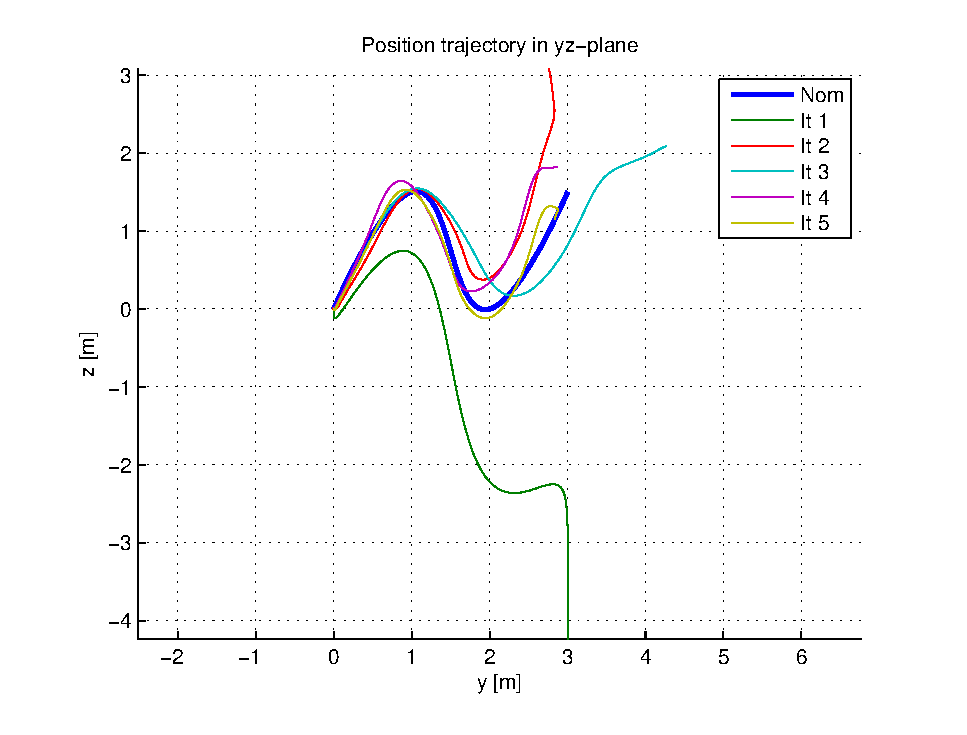
\includegraphics[scale=0.50]{ILCgravity_yz.eps}	
\caption{Tracking results for ILC under gravity mismatch}
\label{fig:ilc_x1}
\end{figure}

Figure \ref{fig:ilc_x1} shows the convergence of the trajectory over iterations. Note that adding more noise reduces the performance, i.e. ILC requires more iterations to converge.

\begin{figure}
\center
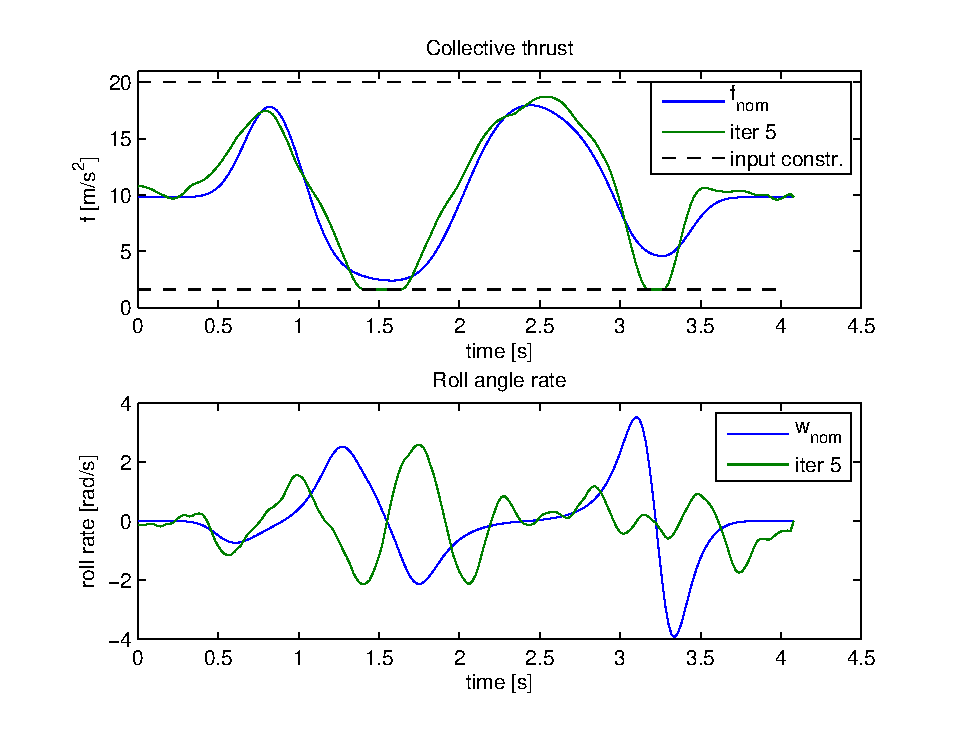
\includegraphics[scale=0.50]{ILCgravity_us.eps}	
\caption{Control inputs over ILC iterations}
\label{fig:ilc_u1}
\end{figure}

Figure \ref{fig:ilc_u1} shows the change in the control inputs needed to accommodate the gravity mismatch. Only the final input is shown, for better visibility.

%CGP-UCB results
Figures \ref{fig:res1_g} - \ref{fig:res2_g}, CGP-UCB learning results again for the same system dynamics. It is assumed here that the cost difference to be learned, as a function of $x := (\context;\sysInput)$, is a realization (or a drawn sample) of a GP with:

\begin{align}
f(x) &\sim \mathcal{N}(\mu(x), k(x, x')) \label{GP prior for quadrocopter} \\
\mu(x) &= 0 %\beta_{\mu}\context + \beta_0 
\label{mean hyperparameters for quadrocopter} \\
k(x, x') &= \sigma_{s}^{2}k_u(\sysInput, \sysInput')k_c(\context, \context') + \sigma_{n}^{2}\delta_{xx'} \label{kernel} \\ 
k_u(\sysInput, \sysInput') &= \sysInput^{\mathrm{T}}\Lambda_{u}^{-2}\sysInput' \label{action kernel} \\
k_c(\context, \context') &= \exp(-\frac{1}{2}(\context-\context')^{\mathrm{T}}\Lambda_{c}^{-2}(\context-\context')) \label{context kernel}
\end{align}

Diagonal matrices $\Lambda_{u}$ and $\Lambda_{c}$ transform anisotropic coordinates into isotropic coordinates or they can be motivated from Automatic Relevance Determination (ARD) point of view where $\Lambda_{u}^{2}$ and $\Lambda_{c}^{2}$ encode the relevance of inputs and contexts, respectively \cite{GPbook}.
This means that hyperparameter estimation is performed with a model structure consisting of 
%a linear mean with intercept and 
a composite kernel that is the product of a linear ARD kernel for the input space $\mathrm{U(t)}$ and a Squared Exponential (SE) ARD kernel for the context space $\mathrm{C}$. For quadrocopter dynamics (\ref{quadrocopterDynamics}) this transforms the problem into a QP-program, see section \ref{ControlAffine}.

\begin{figure}
\center	
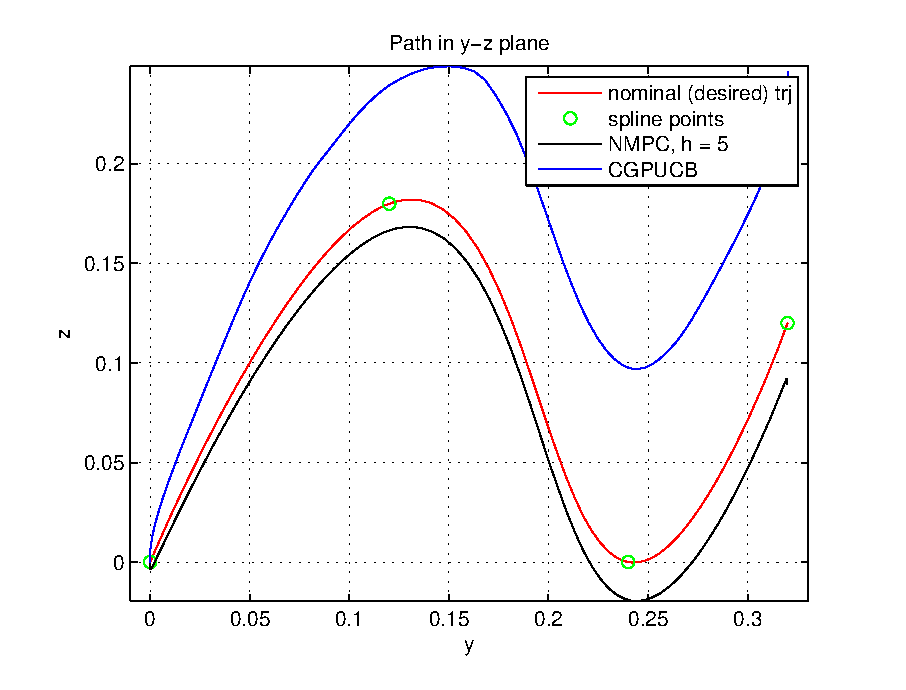
\includegraphics[scale=0.40]{res1_g.eps}	
\caption{Gravity mismatch: tracking results of the first run}
\label{fig:res1_g}
\end{figure}

\begin{figure}
\center
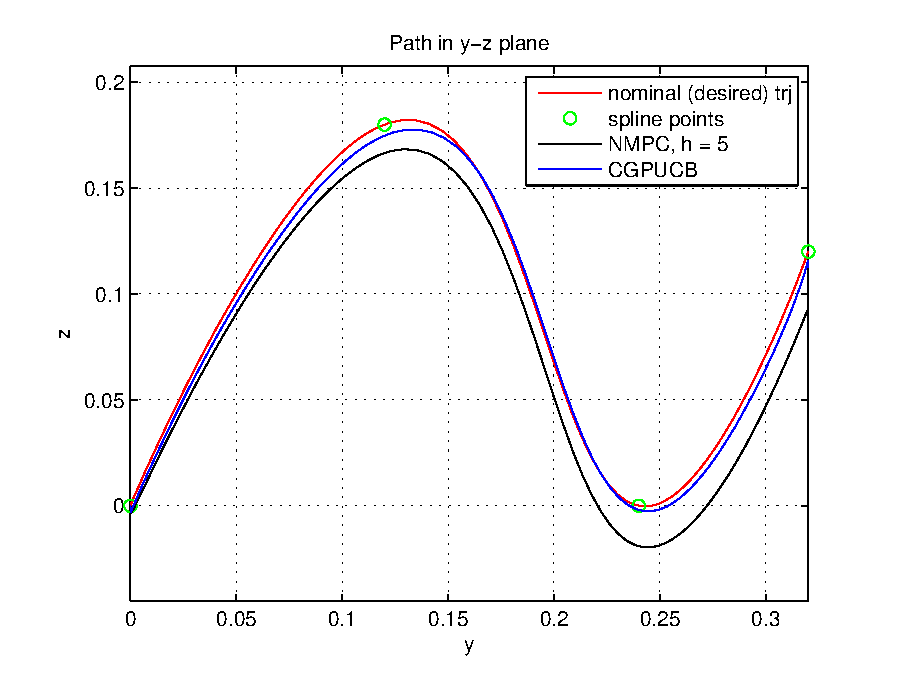
\includegraphics[scale=0.40]{res2_g.eps}	
\caption{Gravity mismatch: tracking results of the third run}
\label{fig:res2_g}
\end{figure}

\begin{figure}
\center
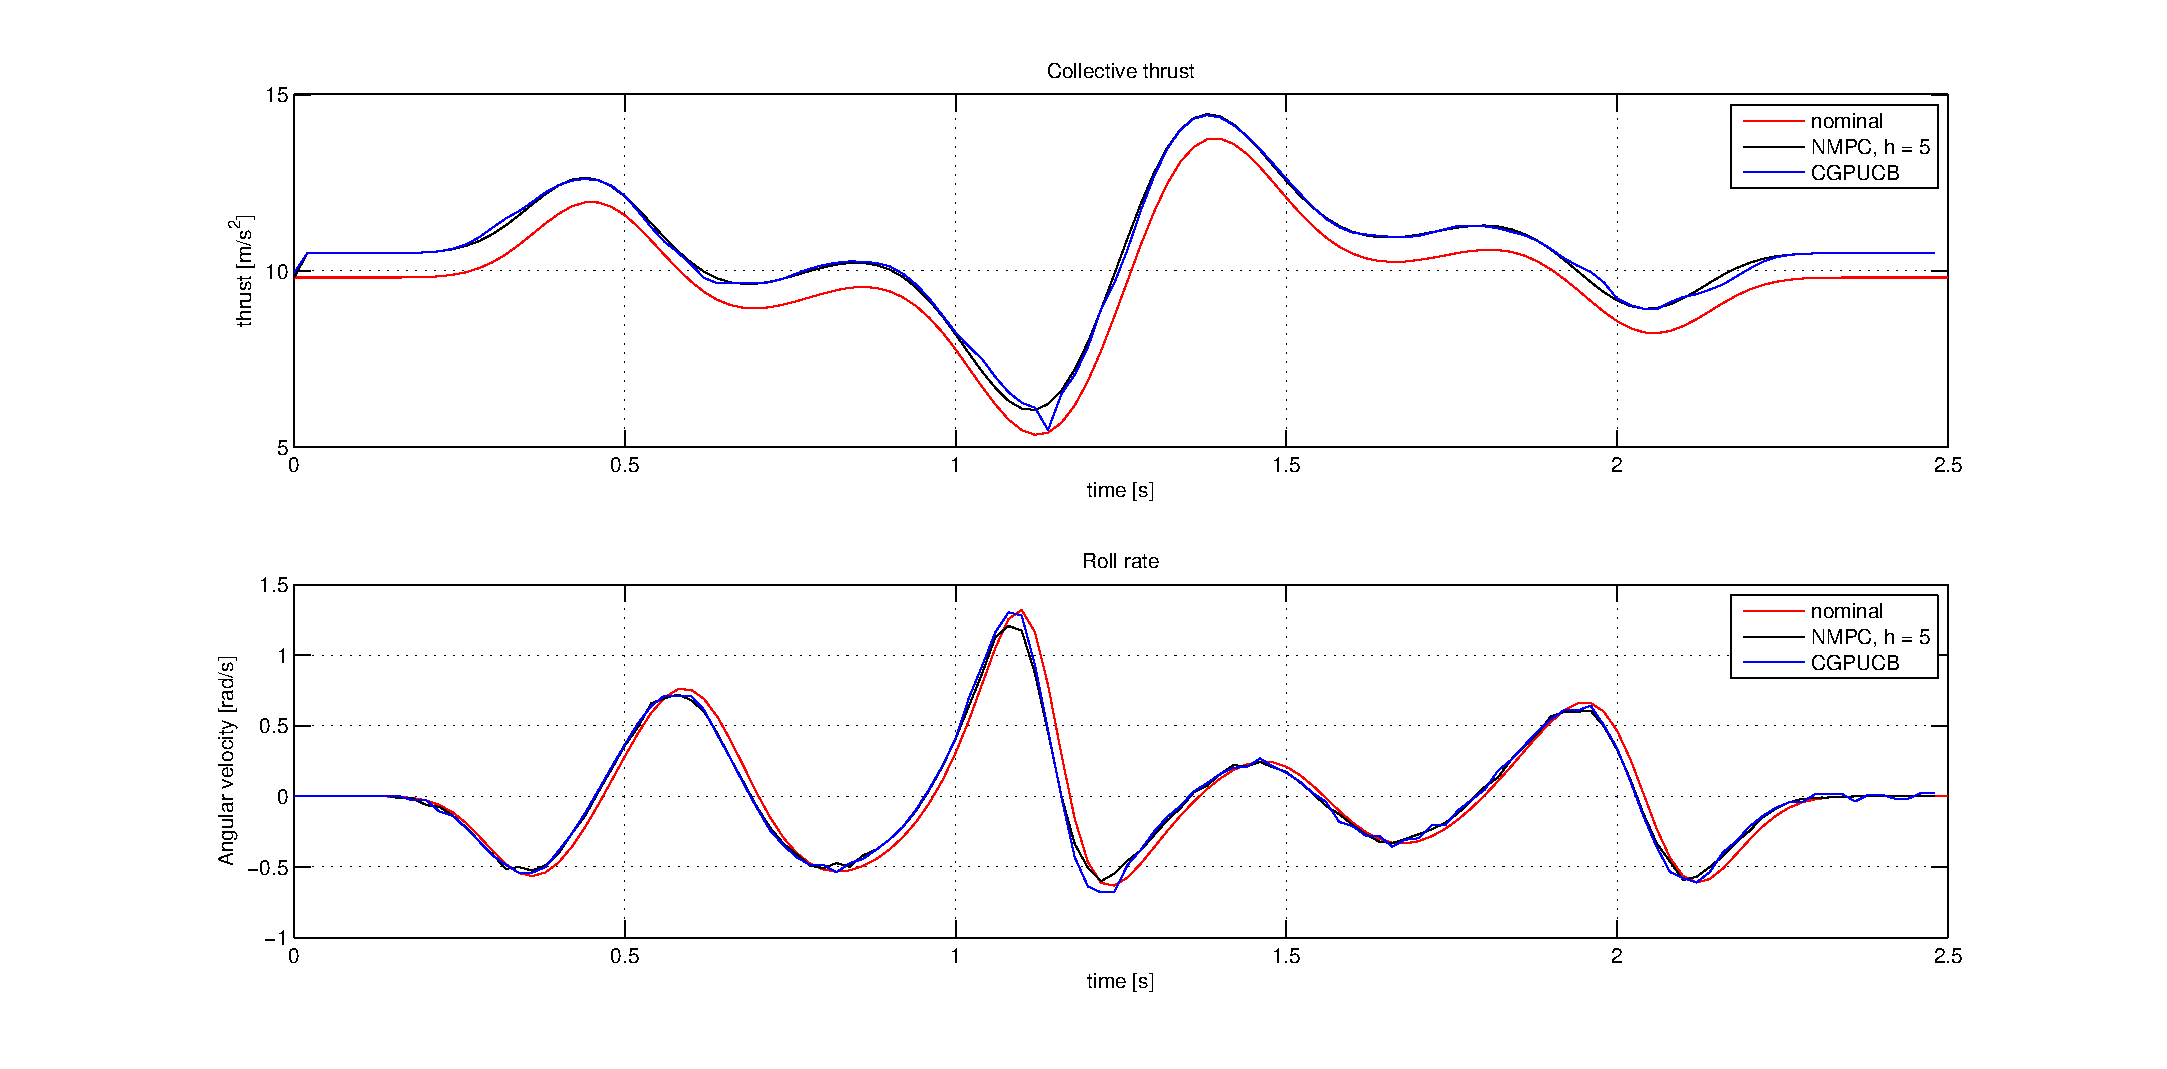
\includegraphics[scale=0.20]{inp1_g.eps}			
\caption{Gravity mismatch: control inputs for the third run}
\label{fig:inp1_g}
\end{figure}

Figure \ref{fig:inp1_g} shows the applied control signals for the third run shown in figure \ref{fig:res2_g}. Sum of squares (SSE) error for the three trials are shown in \ref{SSE_errors}. They clearly show that the method can outperform MPC when disturbances in the form of unknown dynamics are present. $Q$ matrix was taken to be diagonal, with entries $(1,1,1,1,0.01)$.

\begin{table}[h!t]
% increase table row spacing, adjust to taste
\renewcommand{\arraystretch}{1.3}
\caption{SSE errors}
\label{SSE_errors}
\centering
\begin{tabular}{cc}
\textbf{Method / Iteration No.} & SSE \\
\hline
MPC, horizon = 5 & 0.042284 \\
CGP-UCB, trial 1 & 0.914764 \\
CGP-UCB, trial 2 & 0.003622 \\
CGP-UCB, trial 3 & 0.001949 
\end{tabular}
\end{table}

\subsection{Wind Disturbance}
In the second case, we consider a constant horizontal wind force with $P_{wind} = 50 \mathrm{N/m}^{2}$ and $A = 0.16 \mathrm{m}^2$ whose dynamics is analyzed in Example 2, \eqref{example2General}. The cost function difference is given explicitly in equation \eqref{QuadTheta0}. ILC is unable to compensate for this type of disturbance dynamics, as can be seen in Figure \ref{fig:ilc_x2}. 

\begin{figure}
\center	
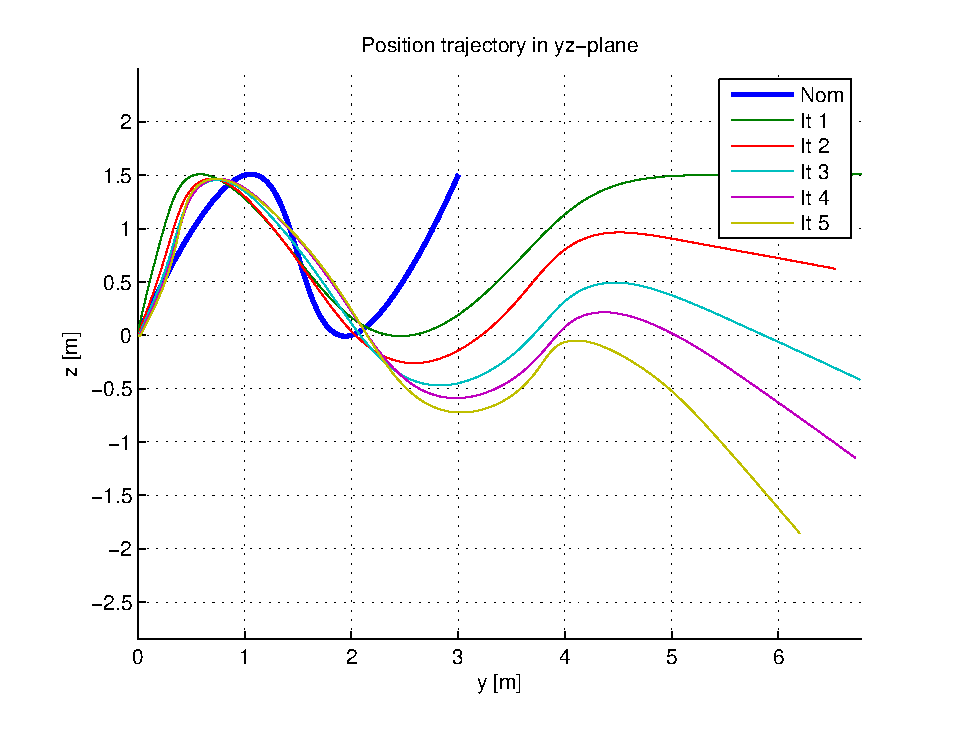
\includegraphics[scale=0.40]{ILCwind_yz.eps}	
\caption{Tracking results for ILC under wind disturbance}
\label{fig:ilc_x2}
\end{figure}

Here transfer learning is shown to take place between two different trajectories. Figure \ref{fig:res1_wind} shows the tracking result for the first trajectory at first iteration. In the second iteration, the trajectory is rotated by 90 degrees. Figure \ref{fig:res2_wind} shows the tracking results for this second trajectory. Comparing with an alternative initial run of the wave trajectory, shown in Figure \ref{fig:res3_wind}, we can clearly see knowledge transfer taking place. This has been accomplished by transferring the costs learned during the first trajectory runs to the second trajectory, using the smoothing provided by the squared exponential kernel for the contexts. However, showing convergence while doing transfer learning over different trajectories, especially in the case of big disturbances, is difficult. There are also issues complicating the application of this approach to transfer learning:

1. The $Q$ matrix. $Q$ was taken to be diagonal with entries $(1,0,0,0,0.01)$. Notice that the variations in the fifth state $\theta$ are only penalized by $0.01$. This causes the applied $w_{x}$ inputs to be very non-smooth. However this lowering of the $\theta$ penalty is necessary to secure learning to track the trajectory with a \emph{single} stage cost. Rolling out the learned cost (stage cost mean) over a horizon should help to make the applied inputs more smooth.

2. Matrix inversion. It takes more trials in general, to show transfer learning, than to show convergence for a single trajectory. But as trials increase, it takes much more time to invert (or use backlash on) the covariance matrix. Reduced rank approximations of the covariance matrix can be applied to speed up the inversion. Mining the past data for \emph{relevant} contexts and inputs then, is a critical part of showing transfer learning.

3. Converging trajectories. Aside from ensuring stability, constructing converging trajectories around the trajectory can help to increase knowledge transfer. By generating trajectories offline perhaps, or perhaps by guiding the process online, one can try to improve the speed of transfer learning. This is because by following the state space around a trajectory, learning can become much more robust to changes in the objective, i.e. the trajectory itself. For the simulations shown in this section, implementing a converging trajectory method $H$, can help to produce better results.

\begin{figure}
\center	
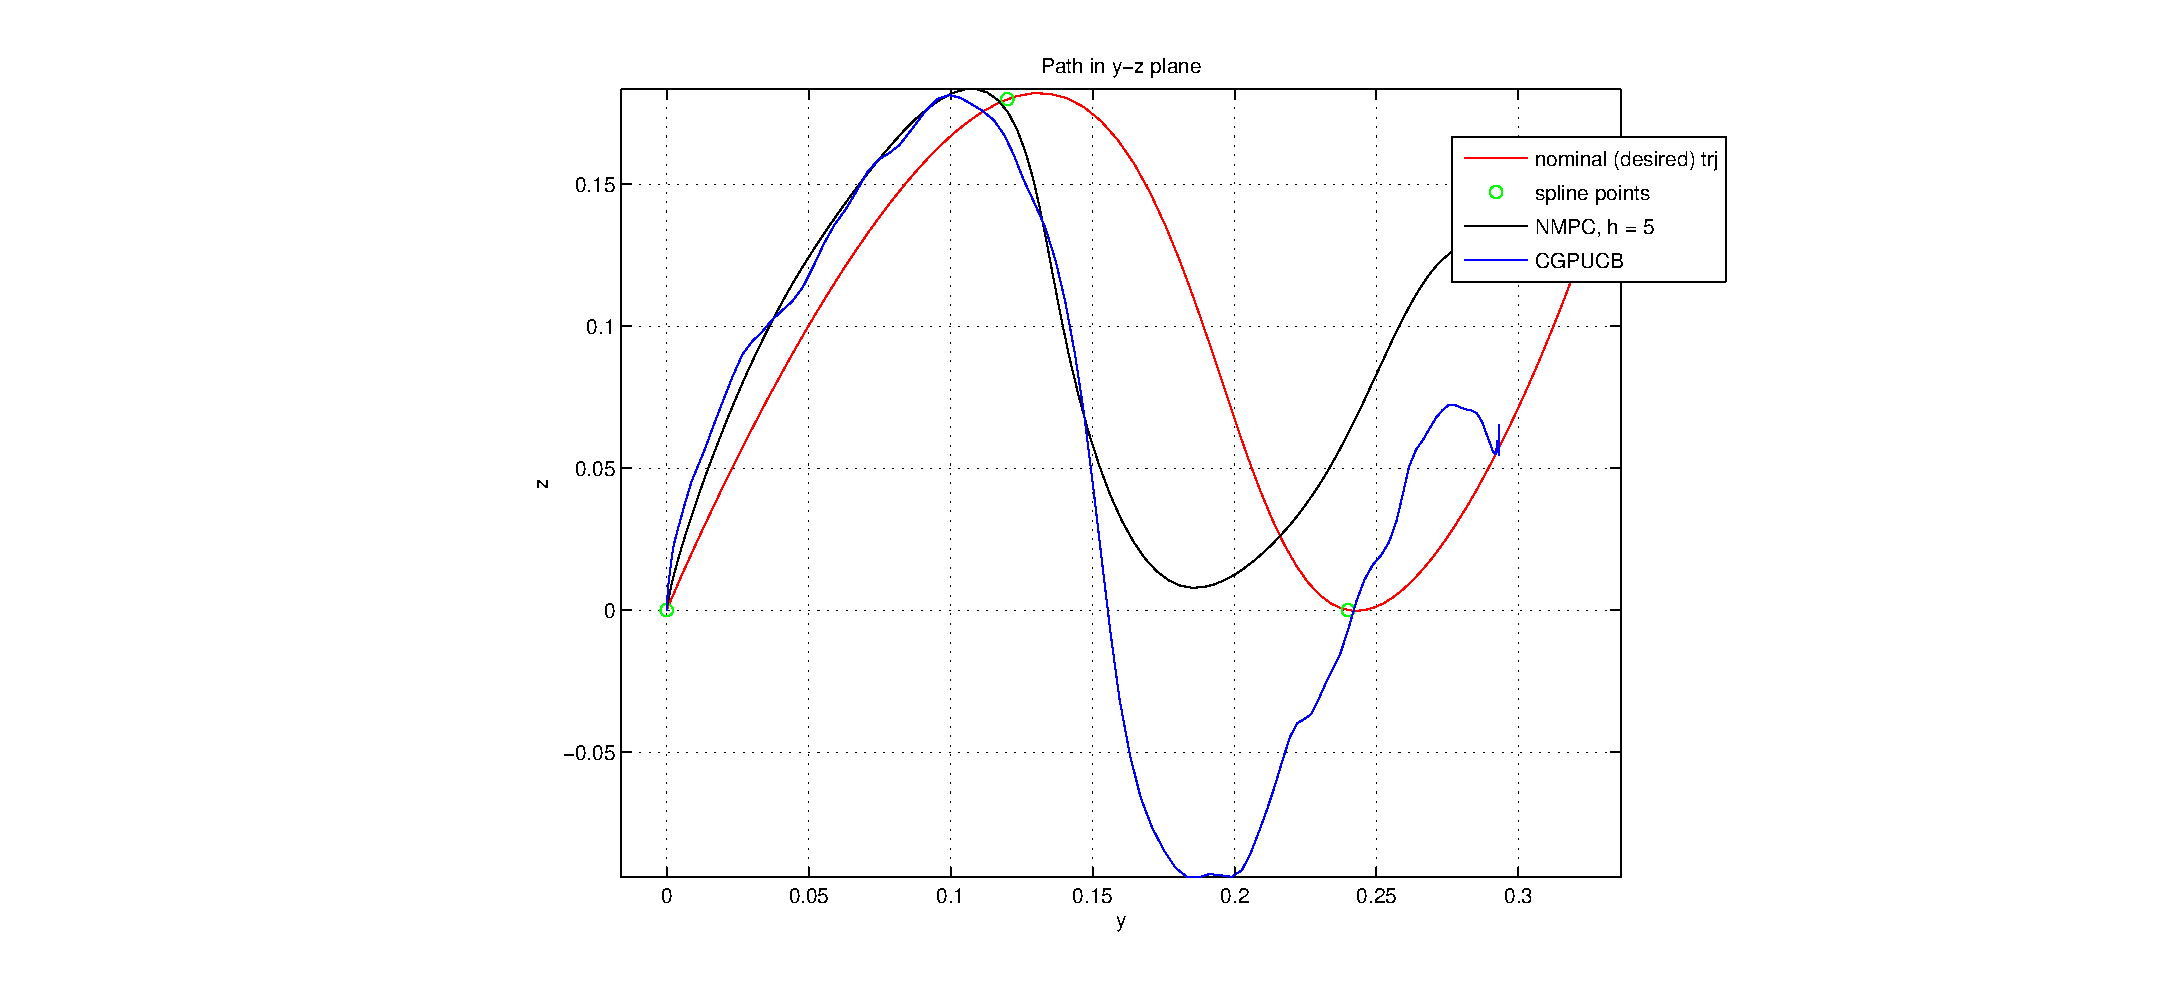
\includegraphics[scale=0.40]{res1_wind.eps}	
\caption{Tracking result of the first trajectory}
\label{fig:res1_wind}
\end{figure}

\begin{figure}
\center
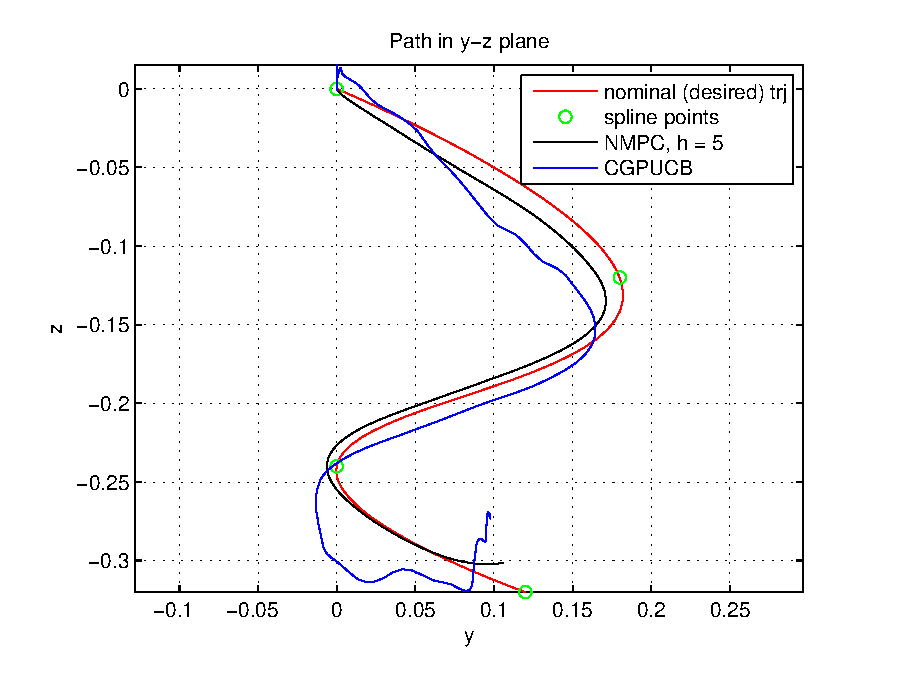
\includegraphics[scale=0.40]{res2_wind.eps}	
\caption{Tracking result of the second trajectory}
\label{fig:res2_wind}
\end{figure}

\begin{figure}
\center
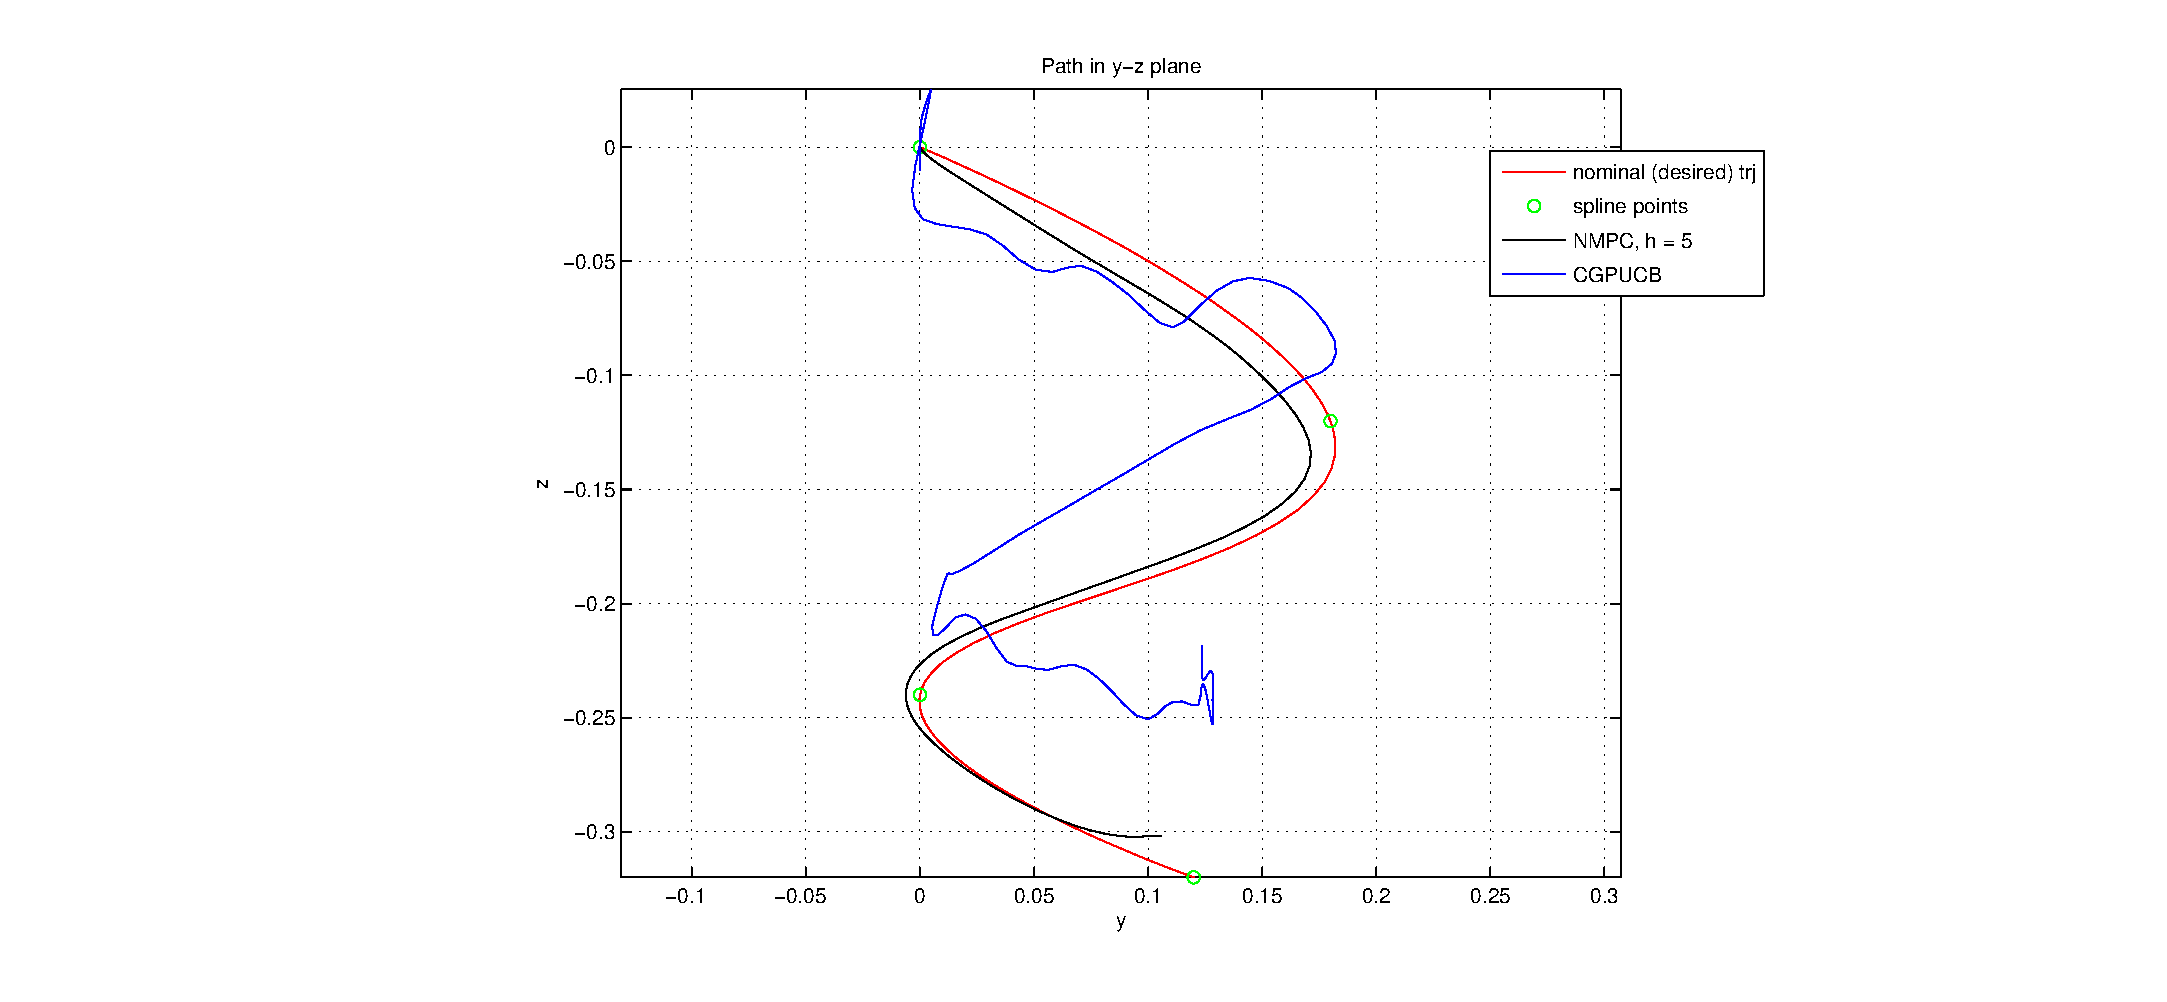
\includegraphics[scale=0.40]{res0_wind.eps}	
\caption{Alternative initial run of the second trajectory}
\label{fig:res3_wind}
\end{figure}